\documentclass[11pt,letterpaper,en-US]{article}

\usepackage{basicstyle}

\title{CS6378 Advanced Operating System Project 2 \\Design Document}

\author{Hanlin He (hxh160630)}

\begin{document}
\maketitle

\section{Introduction}
This document describes the development process of the project.
It generally consists of six parts:
requirement analysis,
use cases,
domain model,
class diagram,
communication protocol design
and program output.

\section{Requirement}
\begin{enumerate}
    \item The system should consists of 7 data servers
        and 5 clients.
    \item Clients should be able to store content on servers,
        and each content should have 3 replica on 3 different servers.
        Each content should have a distinct ID.
    \item The system should provide a hash function so that
        a content with certain ID will always be store on 3
        specific servers.
    \item A client should be able to randomly choose any of the
        three replicas of an object when it wishes to read the
        value of the object.
        If a client tries to read an object that is not present,
        the operation should return with an error code.
    \item When a client wishes to update/insert an object into
        the data repository, it should be able to successfully
        perform the operation on at least two, and if possible
        all the three servers that are required to store the object.
    \item If a client is unable to access at least two out of the
        three servers that are required to store an object, then
        the client does not perform updates to any replica of
        that object.
    \item If two or more clients try to concurrently write to
        the same object and at least two replicas are available,
        the writes must be performed in the same order at all
        the replicas of the object.
\end{enumerate}

\section{Use Cases}
\subsection{Use Case Diagram}
First, consider the system as a black box,
in user's perspective, there are only two scenarios: read and write in the system.
The use case diagram is shown in \cref{ucdori}
\begin{figure}[!htb]
    \caption{Use Case Diagram Consider the System as Black Box}
    \label{ucdori}
    \centering
    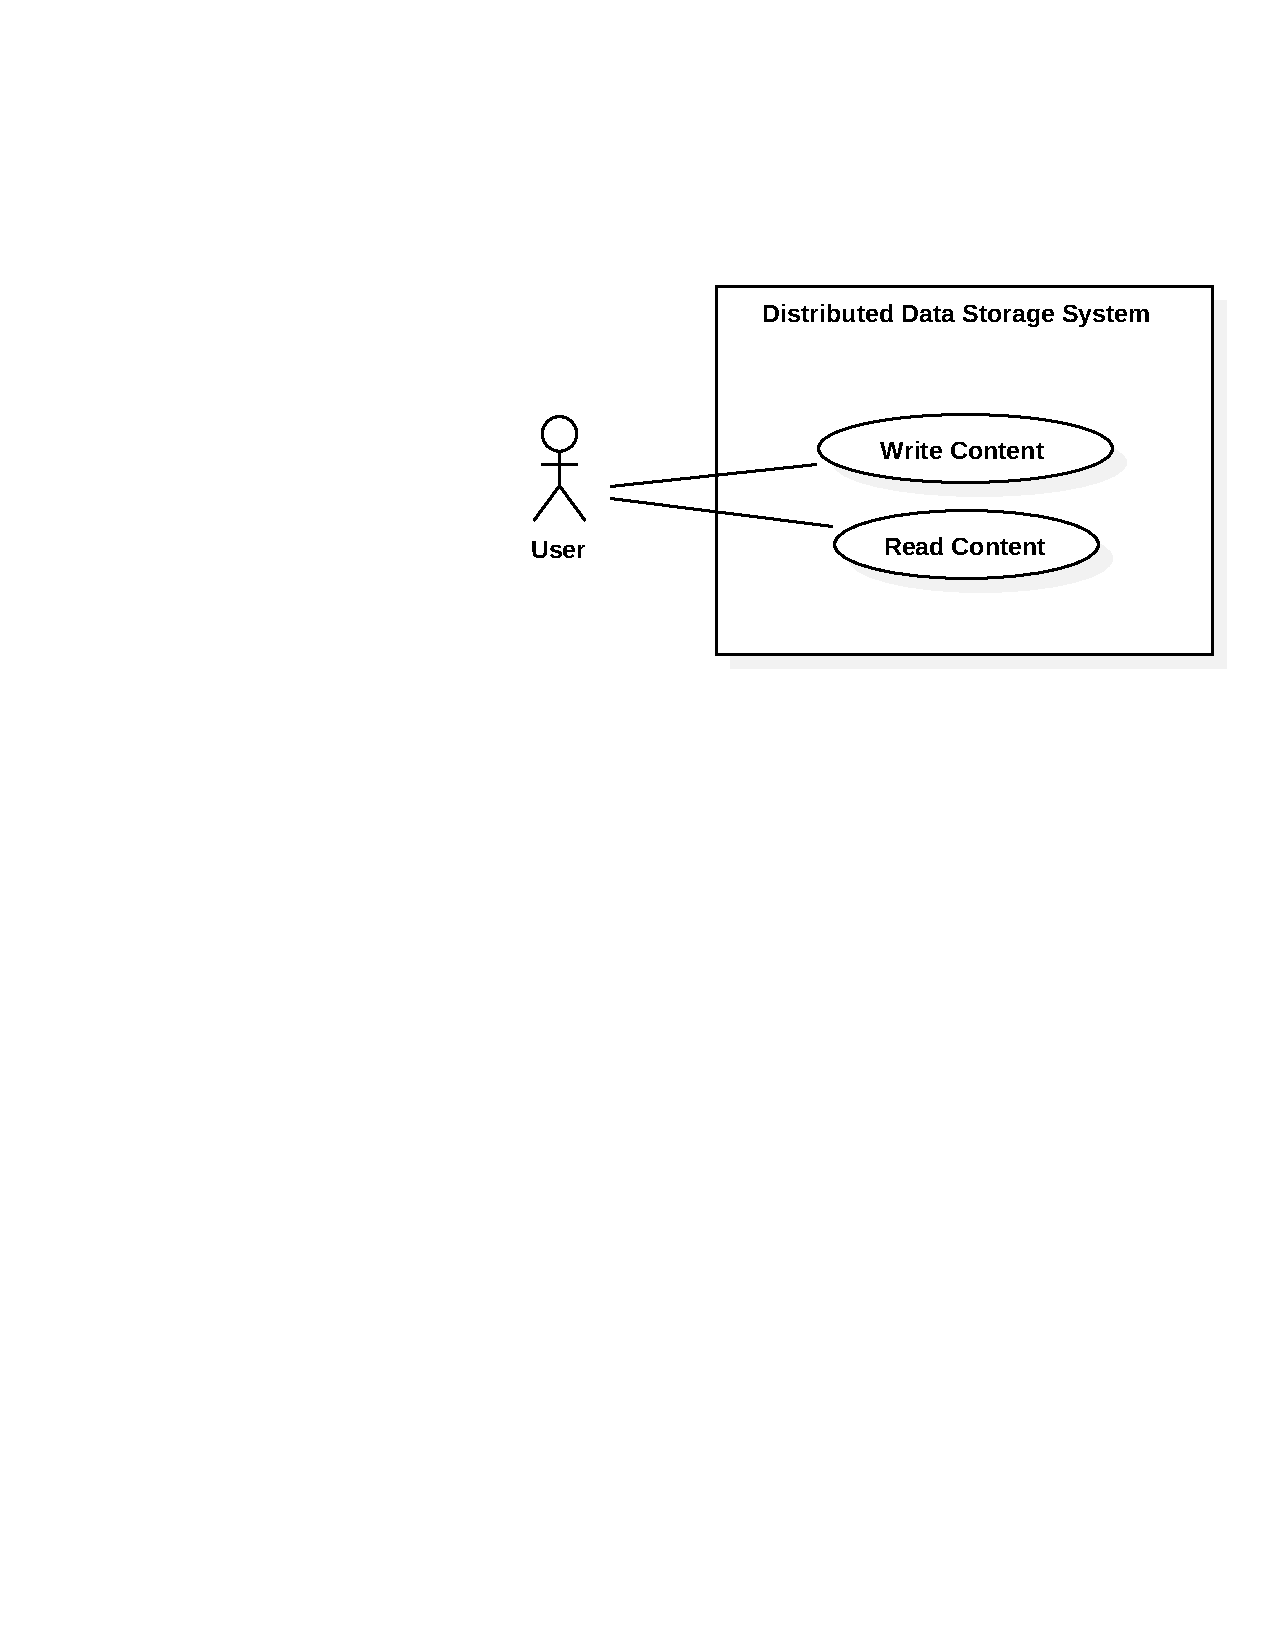
\includegraphics[width = 0.6\textwidth]{usecaseori}
\end{figure}

Furthermore, if we divide the system into server and client,
the client is the representative of the system in user's view, i.e.
the black box in previous diagram.
Now consider the server as a black box and client as the user.
The scenarios remain the same.

\subsection{Use Case Text}
\subsubsection{Use Case: Write Object}
\begin{tabularx}{\textwidth}{>{\bfseries}lX}
    Use Case Name: & Write Content\\
    Scope: & Distributed Storage System\\
    Level: & User Goal\\
    Actors: & User\\
    Stakeholders: & User - Specify content ID,\\
                  & System - Correctly store the content. \\
\end{tabularx}\\
\begin{tabularx}{\textwidth}{X}
    \textbf{Main Flow (Success)}
    \begin{enumerate}[label={\arabic*.}]
        \item The system indicates that it's ready to accept command.
        \item The user enters the write command, specifying the target
            server, the content id and the value to be written.
        \item The system displays the write success message.
        \item Repeat 2-3 until the user terminate the program.
        \item The use case ends successfully.
    \end{enumerate}
\end{tabularx}\\
\begin{tabularx}{\textwidth}{X}
    \textbf{Extensions}
    \begin{itemize}
        \item[*a.] At any time, user exit the system.
            \begin{enumerate}[label={\arabic*.}]
                \item The system goes back to the process, waiting for user to operate.
            \end{enumerate}
    \end{itemize}
\end{tabularx}\\
\begin{tabularx}{\textwidth}{X}
    \textbf{Alternate Flow - More than one server unavailable, write operation fail.}
    \begin{itemize}
        \item[3a.] The system display a write error message and wait for user next command.
    \end{itemize}
\end{tabularx}\\
\begin{tabularx}{\textwidth}{X}
\textbf{Post Conditions (Success Guarantee)}\\
\textbf{Successful Completion} \\
\qquad The system correctly store the content on at least two server.\\
\textbf{Failure Condition} \\
\qquad The system store the content on only one server, or the values of three replicas on each normal server is different.\\
\end{tabularx}

\subsubsection{Use Case: Read Object}
\begin{tabularx}{\textwidth}{>{\bfseries}lX}
    Use Case Name: & Read Content\\
    Scope: & Distributed Storage System\\
    Level: & User Goal\\
    Actors: & User\\
    Stakeholders: & User - Specify content ID
\end{tabularx}\\
\begin{tabularx}{\textwidth}{X}
    \textbf{Main Flow (Success)}
    \begin{enumerate}[label={\arabic*.}]
        \item The system indicates that it's ready to accept command.
        \item The user enters the read command, specifying the target server,
            and the content ID.
        \item The system displays the value of the content.
        \item Repeat 2-3 until the user terminate the program.
        \item The use case ends successfully.
    \end{enumerate}
\end{tabularx}\\
\begin{tabularx}{\textwidth}{X}
    \textbf{Extensions}
    \begin{itemize}
        \item[*a.] At any time, user exit the system.
            \begin{enumerate}[label={\arabic*.}]
                \item The system goes back to the process, waiting for user to operate.
            \end{enumerate}
    \end{itemize}
\end{tabularx}\\
\begin{tabularx}{\textwidth}{X}
    \textbf{Alternate Flow - The selected server is not working.}
    \begin{itemize}
        \item[3a.] The system display a read error message and wait for user next command.
    \end{itemize}
\end{tabularx}\\
\begin{tabularx}{\textwidth}{X}
    \textbf{Alternate Flow - The selected content does not exist on server.}
    \begin{itemize}
        \item[3a.] The system display a read error message and wait for user next command.
    \end{itemize}
\end{tabularx}\\
\begin{tabularx}{\textwidth}{X}
\textbf{Post Conditions (Success Guarantee)}\\
\textbf{Successful Completion} \\
\qquad The system correctly retrieve the content on server.\\
\textbf{Failure Condition} \\
\qquad The system fail to retrieve the value of specifies content.
\end{tabularx}

\section{Domain Model}
Based on use cases, we can identify the following concept.
\begin{itemize}
    \item Host.
    \item Client.
    \item Server.
    \item VectorTime.
    \item Message.
    \item Content.
\end{itemize}
The corresponding domain model is shown if \cref{domainm}.

\begin{figure}[h]
    \caption{Domain Model}\label{domainm}
    \centering
    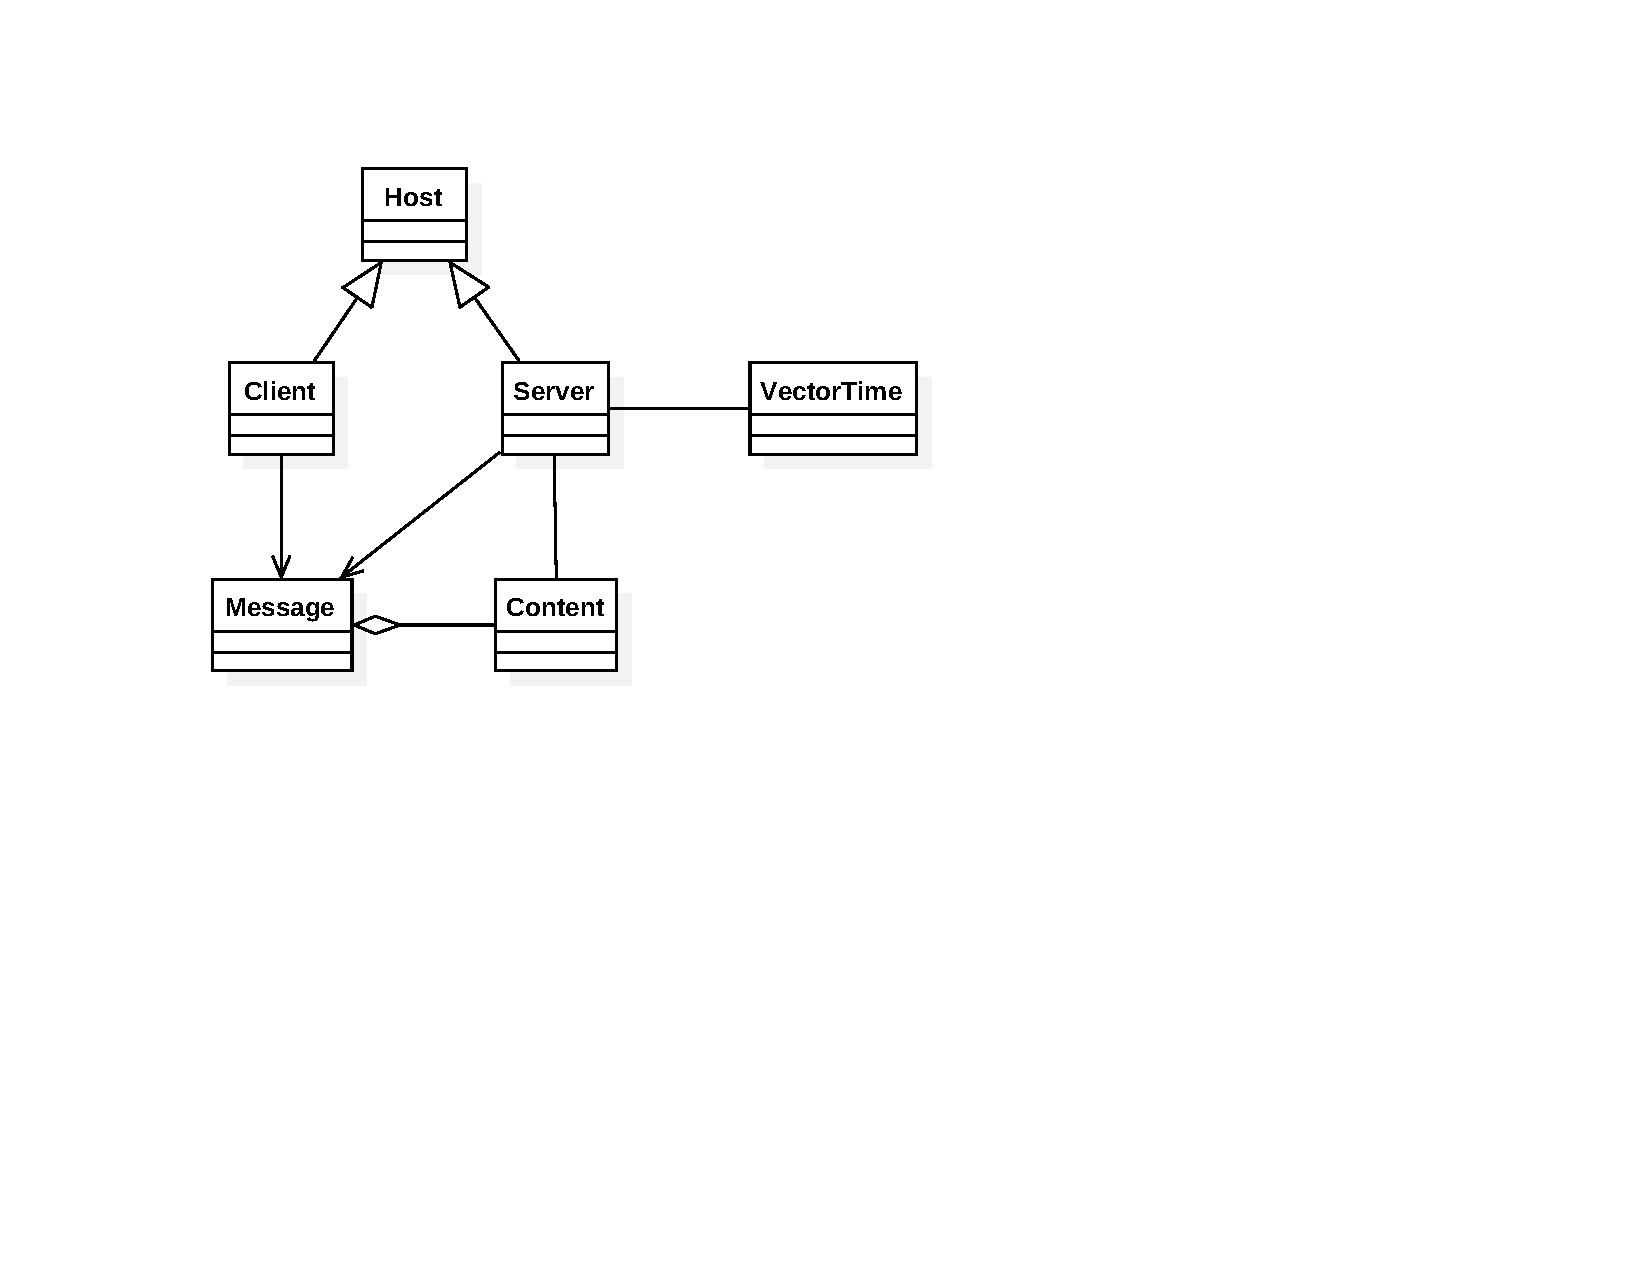
\includegraphics[width=.6\textwidth]{domainmodel}
\end{figure}

The system sequence diagram is basically the same as use case text, so the document will not cover it.

\section{Class Diagram and Specification}
Furthermore analyze the domain model, I derived the class diagram for the system as shown in \cref{classdia}.

\begin{figure}[!hb]
    \caption{Class Diagram}\label{classdia}
    \centering
    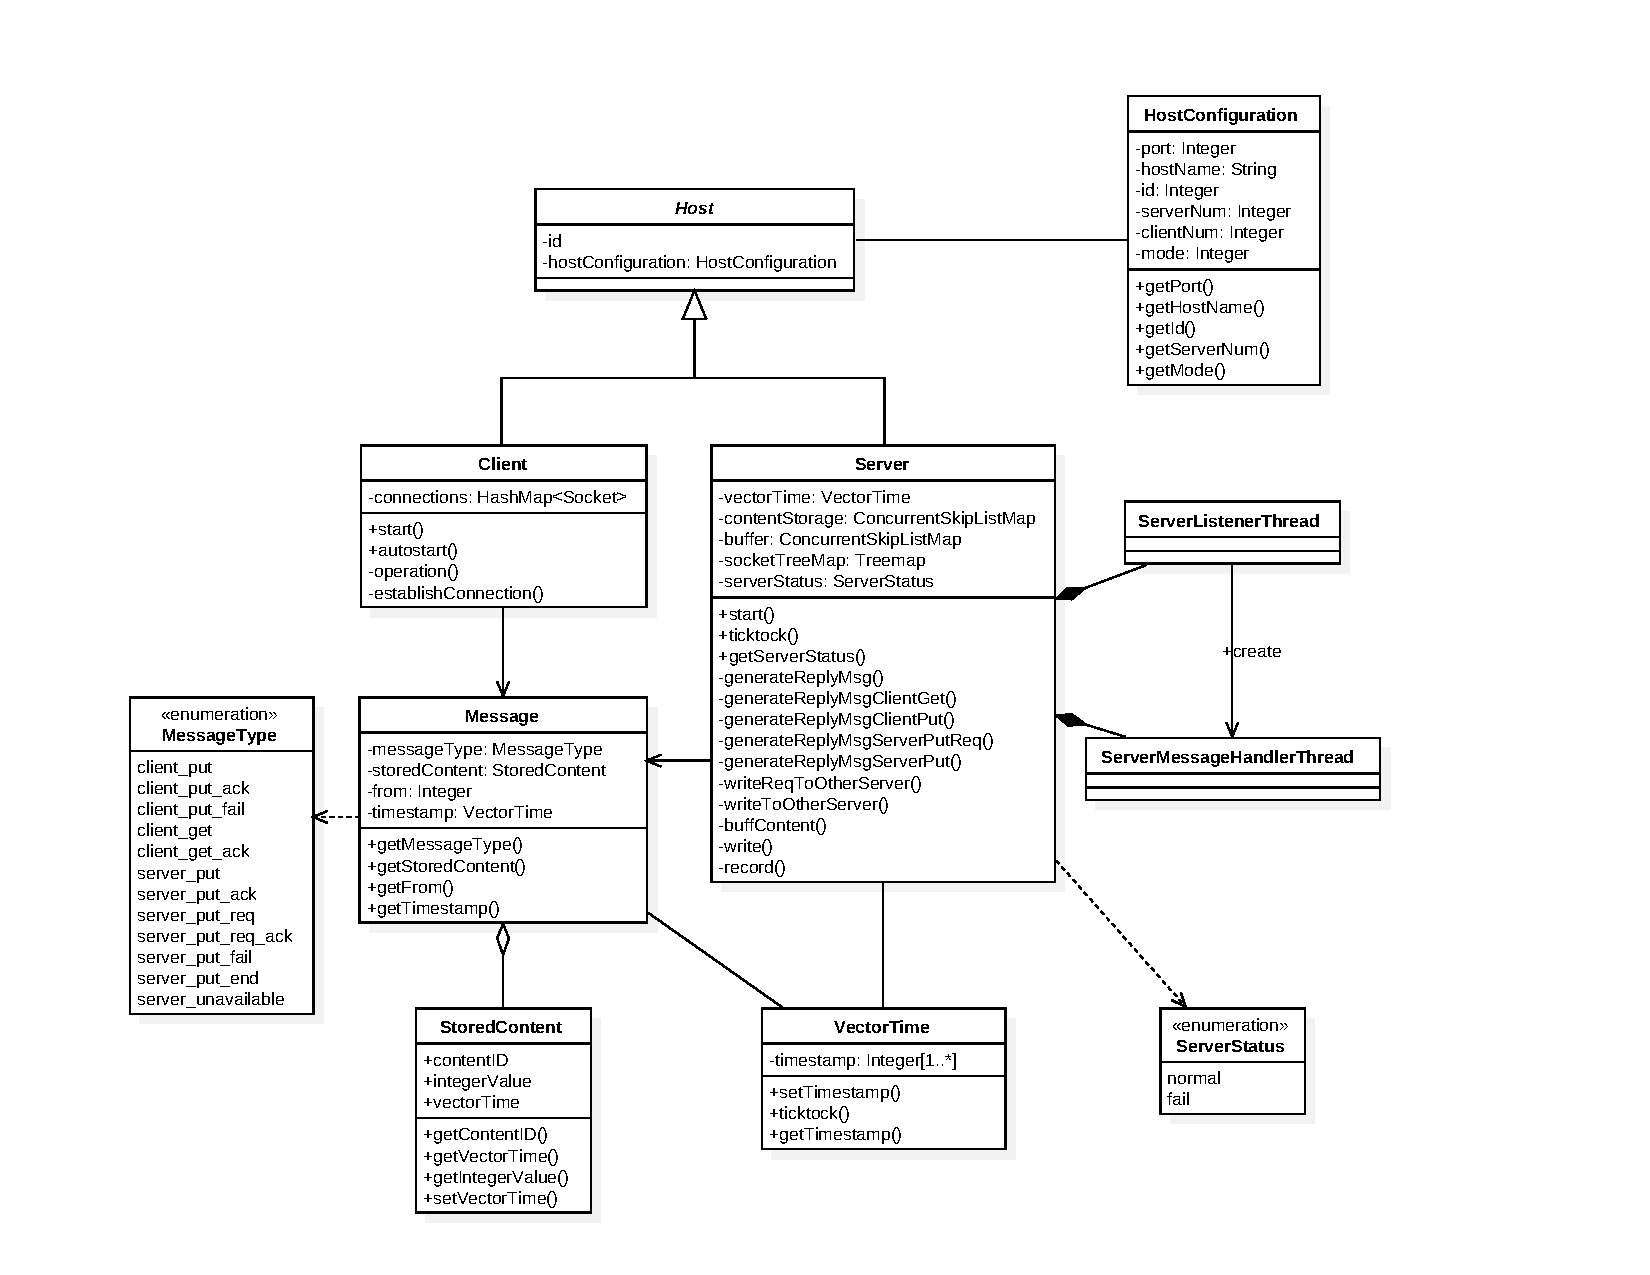
\includegraphics[width=\textwidth]{classdiagram}
\end{figure}

\subsubsection*{Some Specification about the Class Diagram}
\begin{itemize}
    \item \emph{HostConfiguration} class is the configuration read from the file,
        indicating which host with specific acting as client or server,
        and its corresponding working mode.
    \item \emph{Client} the \emph{Server} are basically the specialization of class \emph{Host},
        inheriting the identity variable \emph{id} and configuration \emph{hostConfiguration}.
    \item \emph{VectorTime} is to implement vector clock. It helped to implement the
        ordering of concurrently writing operation.
    \item \emph{StoredContent} is used to represent the object in storage. It uses an
        integer value as key and another integer as value.
    \item \emph{Message} object is data being transfer among the network. Its type reflects
        the operation of the sender. If a message was sent from a client, it would not
        carry the vector timestamp since client does not have that. On the other hand,
        when the message is from a server, it carries the vector timestamp so that the
        other servers may know the causal relation of each message.
\end{itemize}

More detailed information about different message types will be talked about in next chapter.

\section{Inter-Server and Communication Protocol}
\subsection{Inter-Server Sychronization}
There are two choices for selecting the coordinator of the write operation in the system:
\begin{itemize}
    \item The client directly informs three server about the write operation.
        The three server is the quorum for a client.
    \item The client only informs one server about the write operation,
        and let the servers themselves to synchronize.
\end{itemize}
Based on Amazon's Dynamo\cite{amazon1}, the second approach is adopted in this project,
since it guarantee the concurrent write operations of the same content on all servers.

\subsection{Communication Protocol}
The core component of this project is a well-defined communication protocol\cite{liang1}.
The messge type used in this project is list in \cref{mtype}:

\begin{table}[H]
    \caption{Message Type}\label{mtype}
    \centering
    \begin{tabularx}{\textwidth}{>{\ttfamily}lllX}\hline
        \textnormal{Message Type} & From & To & Specification \\\hline
        \detokenize{client_put} & Client & Server & Client specifies the content and its value to update/insert. \\\hline
        \detokenize{client_put_ack} & Server & Client & Server acknowledge the success of write operation. \\\hline
        \detokenize{client_put_fail} & Server & Client & Server informs the client about the failure of write operation. \\\hline
        \detokenize{client_get} & Client & Server & Client specify the content value to be retrieved. \\\hline
        \detokenize{client_get_ack} & Server & Client & Server send the acknowledgment together with the wanted content value. \\\hline
        \detokenize{server_put} & Server & Server & Server informs other servers to commit changes. \\\hline
        \detokenize{server_put_ack} & Server & Server &  Server acknowledge the success of commit operation to the source server. \\\hline
        \detokenize{server_put_req} & Server & Server & Server requests other servers to write a content. \\\hline
        \detokenize{server_put_req_ack} & Server & Server & Server acknowledge that it is ready to write the specific content. \\\hline
        \detokenize{server_put_fai}l & Server & Server & Server informs the source server about the failure of write operation. \\\hline
        \detokenize{server_put_end} & Server & Server & Server informs the target server to close the socket connection. \\\hline
        \detokenize{server_unavailable} & Server & Client & Server informs the client that it is unavailable. \\\hline
    \end{tabularx}
\end{table}

\section{Program Output}
To test the program, I furthermore implemented an automated client to automatically
generate write operation of random content ID ranging from 0 to 9 and value ranging from 0 to 999.

To start the program run the following command on the specific server.

\begin{alltt}
    java Main <Host ID>
\end{alltt}

Upon start, the program would read the configuration file ``all\_nodes.cfg'' in the local directory.
I used the following configuration file:
\begin{alltt}
    7 5
    0 127.0.0.1 20000 0
    1 127.0.0.1 20100 0
    2 127.0.0.1 20200 0
    3 127.0.0.1 20300 0
    4 127.0.0.1 20400 0
    5 127.0.0.1 20500 0
    6 127.0.0.1 20600 0
    7 127.0.0.1 20700 1
    8 127.0.0.1 20800 2
    9 127.0.0.1 20900 2
    10 127.0.0.1 20100 2
    11 127.0.0.1 20110 2
\end{alltt}

The first line indicates the number of server/client in the system (7 servers \& 5 clients).
The following lines indicate the configuration for each host as
\begin{alltt}
    <Host ID> <Host IP> <Host Port as server> <Host Mode>
\end{alltt}
Note that, Host Mode \textbf{0} indicated the host would act as server,
Host Mode \textbf{1} indicated the host would act as normal client,
and Host Mode \textbf{2} indicated the host would act as automated client.


In normal client mode, the command is as follow:
\begin{alltt}
    <Server Choice> <Operation> <Content ID> [New Content Value]
\end{alltt}

The \texttt{Server Choice} could be \emph{a,b,c}, client can choose whichever it want.

The \texttt{Operation} could be \emph{put/get}, if the operation is get, the last parameter
\texttt{New Content Value} is optional.

Based on the configuration, the host 7 is the normal client, so I take the following screen script from host 7.

In the third \texttt{b get 1} command, I typed ``offline'' at server 2, thus the result of \texttt{b get 1} is ``Server Unavailable'',
and the result of \texttt{c put 1 20} is ``Set content 1 as 20 . Result: Success'', since there are still two server available.
And after I set both server 1 and 2 ``offline'', the last \texttt{c put 1 30} command ``Fail'', as there is less than two available server.

\begin{alltt}
> java Main 7
Client start.
Establishing connection to
    Server 0:127.0.0.1:20000... Done.
    Server 1:127.0.0.1:20100... Done.
    Server 2:127.0.0.1:20200... Done.
    Server 3:127.0.0.1:20300... Done.
    Server 4:127.0.0.1:20400... Done.
    Server 5:127.0.0.1:20500... Done.
    Server 6:127.0.0.1:20600... Done.
> a get 1
Content Not exist.
> a put 1 10
Set content 1 as 10 . Result: Success
> b get 1
10
> c put 1 20
Set content 1 as 20 . Result: Success
> b get 1
20
## entering ``offline'' at server 2
> b get 1
Server Unavailable.
> c put 1 20
Set content 1 as 20 . Result: Success
## entering ``offline'' at server 1 and 2
> c put 1 30
Set content 1 as 30 . Result: Fail
\end{alltt}

The server would record a log file at home directory as follow:
\begin{footnotesize}
\begin{alltt}
Content 6 was modified from null    to 320      by node 0   at 2017-03-30 23:07:59.450
Content 1 was modified from null    to 576      by node 2   at 2017-03-30 23:08:00.071
Content 1 was modified from 576     to 10       by node 7   at 2017-03-30 23:08:02.073
\end{alltt}
\end{footnotesize}

\pagebreak
\begin{thebibliography}{2}
\bibitem{amazon1}
  Giuseppe DeCandia, Deniz Hastorun, Madan Jampani, Gunavardhan Kakulapati, Avinash Lakshman, Alex Pilchin, Swaminathan Sivasubramanian, Peter Vosshall and Werner Vogels,
  \emph{Dynamo: Amazon’s Highly Available Key-value Store}
  Amazon.com.
\bibitem{liang1}
  Jun Liang(https://github.com/JunLiang), Xue Ning,
  \emph{Design},
  Github, 2014.
\end{thebibliography}
\end{document}


